\documentclass[12pt]{article}
\usepackage{xcolor}
\usepackage{booktabs}
\usepackage{csquotes}
\usepackage{langsci-gb4e}
\usepackage{hyperref}
\hypersetup{
    colorlinks=true,
    linkcolor=blue,
    filecolor=magenta,
    citecolor=blue,      
    urlcolor=cyan,
    pdftitle={grammaticality},
    pdfpagemode=FullScreen,
}
\usepackage[style=langsci-unified,backend=biber]{biblatex}
\addbibresource{refs.bib}
\usepackage{amsmath}
\usepackage{amssymb}
\usepackage{tcolorbox}
\usepackage{tikz}
\usepackage{pgfplots}
\pgfplotsset{compat=1.18}


\usepackage{microtype}
\usepackage{float}
\usetikzlibrary{arrows.meta,shapes,positioning}
\usepackage{longtable}

\usepackage{orcidlink}

% Define only used colors
\definecolor{lsLightBlue}{RGB}{201,233,246}
\definecolor{lsDOIGray}{RGB}{0,0,0}

% Define upright subscripts
\newcommand{\listener}{\mathrm{L}}

\title{Grammaticality de-idealized\\[4pt]
       \large Lingbuzz preprint v0.3\\[6pt]
       \normalsize \url{https://github.com/BrettRey/Grammaticality-de-idealized-v2}}
\author{Brett Reynolds \orcidlink{0000-0003-0073-7195}\\Humber Polytechnic \& University of Toronto
\thanks{I used ChatGPT o3-pro and Claude Opus 4 in drafting this version of the paper.\\This work is licensed under CC-BY 4.0}}
\date{\today}

\begin{document}
\maketitle

\begin{abstract}
\small
Speakers reject *\textit{I've finished it yesterday} (aspect semantics clash) yet accept the semantically odd \textit{Colorless green ideas sleep furiously} (no morphosyntactic clash). They block *\textit{Which did you buy car?} categorically, while linguists judge the unreadable centre‑embedding \textit{The rat the cat the dog chased killed ate the cheese} ``grammatical".  
The Morphosyntactic–Meaning Model of Grammaticality (MMMG) aims to explain such contrasts by treating grammaticality as the stability of community‑specific form–meaning pairings, not as autonomous syntax or raw frequency.

Five interacting components decide an utterance's status:  
(1) conventional morphosyntactic--meaning pairings;  
(2) compatibility between those meanings and contextual meaning;  
(3) incremental‑processing limits;  
(4) degree of community entrenchment;  
(5) categorical structural bans.

MMMG separates objective grammaticality \(G(u)\) from the subjective feeling of ungrammaticality \(F(u)\), showing why processing overload can make grammatical sentences feel wrong and why compelling semantics can mask true violations.  

A tractable formalization models entrenchment as logistic growth derived from utterance-selection dynamics, predicting S‑curves in language change. The framework yields falsifiable claims about which violations satiate under exposure, how morphosyntactic integration conditions cross‑linguistic variation, and why L2 learners over‑detect errors.  

Grounding grammaticality in community conventions while acknowledging universal processing constraints, MMMG offers a systematic approach to phenomena that elude purely formal or purely usage‑based accounts.
\end{abstract}

\begin{tcolorbox}[colback=lsLightBlue!20,title=Research Programme]
This paper presents a theoretical framework with programmatic predictions for empirical testing. While some supporting evidence exists, systematic validation of the model's quantitative predictions awaits future data collection across the research areas outlined herein.
\end{tcolorbox}

\section{Executive overview}

\paragraph*{Claim.}%
Grammaticality is the \emph{community stability} of morphosyntactic form–meaning pairings.

\paragraph*{Mechanism.}%
Grammaticality emerges from five interacting components:

\begin{enumerate}
    \item \textbf{Morphosyntactic Pairings} — conventional links between morphosyntax and meaning.
    \item \textbf{Contextual Meaning} — composite interpretation drawn from lexical, information-structural, discourse, pragmatic, and socio-pragmatic indexical meanings.
    \item \textbf{Processing Load} — incremental parsing constraints.
    \item \textbf{Entrenchment} — community acceptance.
    \item \textbf{Structural Bans} — categorically blocked configurations.
\end{enumerate}

Together these components produce an objective grammaticality score \(G(u)\) and subjective feeling-of-ungrammaticality score \(F(u)\).

\paragraph*{Why this matters.}%
The framework generates testable predictions about gradient grammaticality, which violations satiate, why some rare patterns remain grammatical, and how ``illusions" of grammaticality and ungrammaticality arise. It explains, for example, why
\begin{itemize}
    \item \textit{I've finished it yesterday} fails (semantic clash),  
    \item centre embeddings \emph{feel} ungrammatical despite being grammatical (processing overload),
    \item the ``comparative illusion'' \emph{feels} grammatical despite being ungrammatical (undetected mismatch),
    \item determiner extractions like \textit{Which did you buy car?} never improve with exposure (structural ban).
\end{itemize}
Objective grammaticality \(G(u)\) and the subjective feeling of error \(F(u)\) can therefore diverge.

\section{Motivation: The impasse in grammaticality theory}

Three long‑standing tensions block a unified account of (un)grammaticality.

\subsection{Categorical rules vs gradient judgements}

\textcite{chomsky1957} cast grammaticality as an all‑or‑nothing property.  
The competence–performance split was meant to park gradience in a separate ``performance" box, yet doing so lets supportive data count as grammar and contrary data count as noise \parencite[71]{schutze2016}.

\ea
\textit{The bread the baker the apprentice helped made is delicious.}
\z
Centre‑embedded relatives are routinely labelled ``grammatical but unprocessable," which merely restates the puzzle: speakers feel them to be wrong.

\subsection{Form vs meaning}

The famous \textit{Colorless green ideas sleep furiously} shows syntactic well‑formedness without plausibility.  The converse also matters:

\ea[*]{\textit{I've finished it yesterday.}}\z
Here the present‑perfect feature [+current relevance] clashes with the \textit{yesterday}'s [+completed past], and speakers reject the sentence.  Construction‑grammar work \parencite{goldberg1995constructions} confirms that morphosyntactic meaning and lexical meaning must cohere, explaining why \textit{She texted him the address} passes while \textit{*She disappeared him the evidence} does not.

\subsection{Universal principles vs community conventions}

Labovian sociolinguistics \parencite{labov1972} shows that grammaticality is community‑relative.  Languages differ not just in lexicon but in which form–meaning pairings are conventionalised.  Usage‑based models capture frequency effects, yet they still face cases where extremely rare patterns remain grammatical and frequent patterns are blocked.

\medskip
These three tensions—categorical vs gradient, form vs meaning, universal vs communal—underline the need for a framework that explains why particular patterns of acceptability recur across speakers and across languages.


\section{Five components of (un)grammaticality}

On the MMMG account, grammaticality emerges as the community stability of morphosyntactic form–meaning pairings. Five interacting components determine this stability:

\subsection{Morphosyntactic pairings within communities}

\begin{tcolorbox}[colback=lsLightBlue!30]
\textbf{Diagnostic}: Does the morphosyntactic form evoke a conventionalised meaning in this community?

\textbf{Example}: \textit{*Can the have running?}~— no viable form–meaning pairing.

\textbf{Counter-example}: \textit{Colorless green ideas sleep furiously}~— odd semantics, but a clear compositional morphosyntactic pairing.
\end{tcolorbox}

Grammaticality fundamentally requires stable, conventionalised pairings between morphosyntactic forms and meanings within a speech community. Communities differ regarding acceptable pairings:

\ea
\textit{Estábamos lifting en el gym.} (Spanish–English bilingual)\\
'We were lifting in the gym.'
\z

This utterance is grammatical in communities accepting code-switching with English progressive forms but not in monolingual Spanish communities.

\subsection{Contextual meaning}

\begin{tcolorbox}[colback=lsLightBlue!30]
\textbf{Diagnostic}: Does the morphosyntactic meaning align coherently with the contextual meaning derived from lexical semantics, information structure, discourse coherence, pragmatic inference, and socio-pragmatic indexicality?

\textbf{Example}: \textit{*I've finished it yesterday}~— present-perfect meaning [+current relevance] clashes with the lexical-discourse meaning of \textit{yesterday} [+completed past].

\textbf{Counter-example}: \textit{I've just finished it}~— coherent alignment with lexical-discourse meaning.
\end{tcolorbox}

Even a well-formed morphosyntactic structure becomes ungrammatical if it misaligns significantly with contextual meanings. Consider:

\ea[*]{\textit{I have 25 years.} \hfill (intended: `I am 25 years old')}
\z

In English, \textit{have + years} fails contextually as an age-expression despite being syntactically viable.

\subsection{Processing load}

\begin{tcolorbox}[colback=lsLightBlue!30]
\textbf{Diagnostic}: Can the sentence be incrementally parsed within memory limits?

\textbf{Example}: \textit{The rat the cat the dog chased killed ate the cheese}~— multiple embeddings overload incremental parsing.

\textbf{Counter-example}: \textit{The rat that the cat killed ate the cheese}~— single embedding, easily processed.
\end{tcolorbox}

High processing demands can induce feelings of ungrammaticality even for objectively grammatical constructions due to parsing constraints.

\subsection{Entrenchment}

\begin{tcolorbox}[colback=lsLightBlue!30]
\textbf{Diagnostic}: Is the pairing conventional and entrenched within the community?

\textbf{Example}: \textit{*We counted three sheeps}~— regular plural blocked by entrenched irregular form.

\textbf{Counter-example}: \textit{We bought three computer mouses}~— recent regularisation already accepted.
\end{tcolorbox}

Even transparent morphosyntactic patterns can fail if not entrenched in a community. For example, the independent relative \textit{whose} remains marginal due to lack of exposure:

\ea[?]{\textit{I saw Joan, a friend of whose was visiting.}}
\z

\subsection{Structural bans}

\begin{tcolorbox}[colback=lsLightBlue!30]
\textbf{Diagnostic}: Does the construction violate a categorically blocked configuration?

\textbf{Example}: \textit{\*Which did you buy \_ car?} — determiner extraction.

\textbf{Counter-example}: \textit{Which car did you buy \_?} — entire NP extraction permitted.
\end{tcolorbox}

Categorical structural bans represent extreme stability biases. While cross-linguistically robust, they are nonetheless emergent rather than strictly universal or innate. The model treats them as a community-entrenchment extreme (effectively zero acceptability), but future work could test their potential malleability under unusual sociolinguistic conditions.

Together, these five components interact systematically to determine the grammaticality of linguistic constructions, accounting both for objective grammaticality and subjective judgments of grammaticality and ungrammaticality.


\section{Quick‑diagnosis decision tree}

The five components can be queried in sequence to classify an utterance on first pass. The tree locates the first component whose failure suffices to render an utterance ungrammatical; later nodes are not evaluated once a zero value is returned.

\begin{figure}[H]
\centering
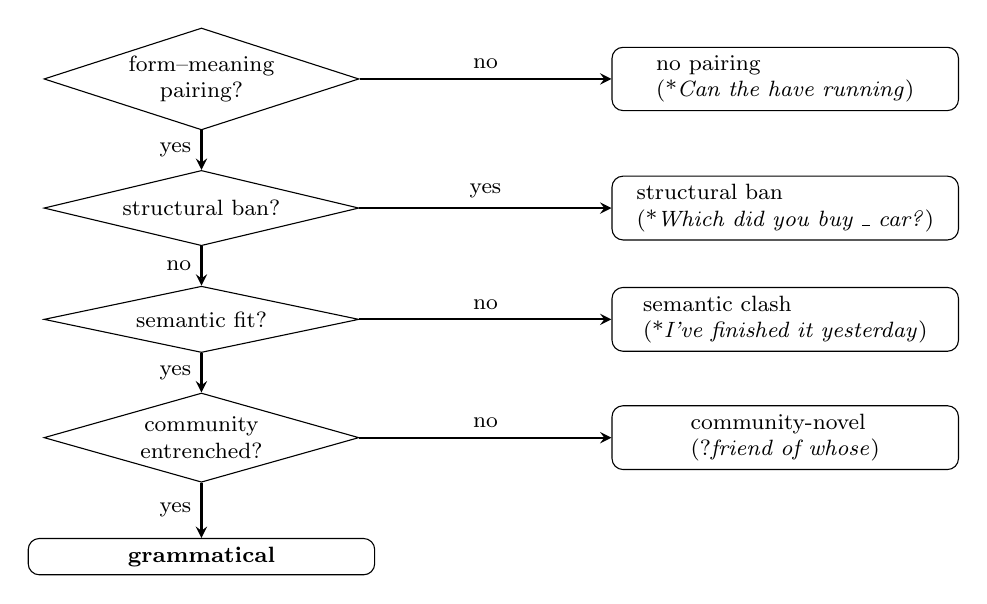
\begin{tikzpicture}[
  font=\footnotesize,                       % smaller text everywhere
  node distance = 0.5cm and 3.2cm,         % tighter vertical gap
  decision/.style = {diamond,
                     aspect=3,              % width : height = 3 : 1  →  flatter
                     draw,
                     align=center,
                     minimum width=4cm,
                     inner sep=1pt},
  outcome/.style  = {rectangle,
                     draw,
                     rounded corners,
                     align=left,
                     minimum width=4.4cm,
                     inner sep=3pt},
  arrow/.style    = {->, >=stealth, thick}
]

\node[decision] (map)  {form–meaning\\pairing?};
\node[outcome , right=of map]  (nonsense) {no pairing\\(*\textit{Can the have running})};

\node[decision, below=of map]  (ban)  {structural ban?};
\node[outcome , right=of ban]  (lbe)  {structural ban\\(*\textit{Which did you buy \_ car?})};

\node[decision, below=of ban]  (sem)  {semantic fit?};
\node[outcome , right=of sem]  (clash) {semantic clash\\(*\textit{I've finished it yesterday})};

\node[decision, below=of sem]  (ent)  {community\\entrenched?};
\node[outcome , right=of ent]  (novel) {community‑novel\\(?\textit{friend of whose})};

\node[outcome , below=0.7cm of ent] (gram) {\textbf{grammatical}};

\draw[arrow] (map)  -- node[above] {no} (nonsense);
\draw[arrow] (map)  -- node[left]  {yes} (ban);
\draw[arrow] (ban)  -- node[above] {yes} (lbe);
\draw[arrow] (ban)  -- node[left]  {no}  (sem);
\draw[arrow] (sem)  -- node[above] {no}  (clash);
\draw[arrow] (sem)  -- node[left]  {yes} (ent);
\draw[arrow] (ent)  -- node[above] {no}  (novel);
\draw[arrow] (ent)  -- node[left]  {yes} (gram);

\end{tikzpicture}
\caption{Decision tree for first‑pass diagnosis.}
\end{figure}


The tree is a heuristic: it points to the first component that fails.  
The underlying grammar is \(G(u)=C^{t} \cdot K(u)\); when any factor is zero, the utterance is objectively ungrammatical even if later nodes would succeed.
\begin{tcolorbox}[colback=lsLightBlue!15]
\textbf{Note.} The tree classifies utterances on the dimension of
\emph{objective grammaticality}. A sentence can pass the tree
($G(u){=}1$) yet yield a negative $F(u)$ if either 
$r(u)$ is high or PCost$(u)$ is large.
\end{tcolorbox}

\section{Notation}

\begin{small}
\begin{longtable}{@{}llp{7cm}@{}}
\caption{Symbols used in the formal model. Type abbreviations: struc.\ = syntactic structure, fea.\ = feature bundle or semantic representation, indic.\ = observed indicator, func.\ = function}\label{tab:notation}\\
\toprule
Symbol & Type & Meaning / construction method \\ 
\midrule
\endfirsthead

\multicolumn{3}{@{}l}{\small\textit{Table~\ref{tab:notation} continued}} \\
\toprule
Symbol & Type & Meaning / construction method \\ 
\midrule
\endhead

\midrule
\multicolumn{3}{r@{}}{\small\textit{Continued on next page}}
\endfoot

\bottomrule
\endlastfoot

\multicolumn{3}{@{}l}{\textit{Utterance-level observables}} \\
$u$ & token & Concrete utterance under evaluation \\
$M(u)$ & struc. & Morphosyntactic parse of $u$ \\
$\mu(u)$ & fea. & Morphosyntactic meaning unpacked from $M(u)$ \\
$\sigma(u)$ & fea. & Composite lexical–pragmatic meaning intended \\
$\text{lex}(u)$ & fea. & Lexical semantic representation of $u$ \\
$\text{discCtx}(u)$ & fea. & Discourse-history information relevant to $u$ \\
$\text{infoCtx}(u)$ & fea. & Information‑structure configuration (topic–comment layout, focus, QUD alignment) \\
$\text{pragCtx}(u)$ & fea. & Pragmatic inference information relevant to interpreting $u$ \\
$\text{idxCtx}(u)$ & fea. & Indexical parameters (speaker, addressee, place, time, etc.) relevant to $u$ \\[0.5em]

\multicolumn{3}{@{}l}{\textit{Semantic interpretation function}} \\
$\varphi$ & func. & Deterministic but underspecified mapping from context and lexical meaning to composite semantic representation \\[0.5em]

\multicolumn{3}{@{}l}{\textit{Evaluation scores}} \\
$K(u)\in[0,1]$ & score & Semantic compatibility of $\mu(u)$ with $\sigma(u)$ \\
$G(u)\in[0,1]$ & score & Objective grammaticality; product defined in Eq.~\eqref{eq:G} \\
$F(u)\in[-1,0]$ & score & Listener's felt ill‑formedness; see Eq.~\eqref{eq:F} \\
$r(u)\in[0,1]$ & score & Diagnostic weight: probability listener detects mismatch between \(\mu(u)\) and \(\sigma(u)\) \\[0.5em]

\multicolumn{3}{@{}l}{\textit{Community latent variable and indicators}} \\
$C^{t}(u)\in[0,1]$ & latent & Community entrenchment at time $t$ \\
$A(u)$ & indic. & Availability in memory (recognition hit rate) \\
$E(u)$ & indic. & Exposure frequency (log corpus count) \\
$P(u)$ & indic. & Production probability (elicitation rate) \\
$S(u)$ & indic. & Social acceptability (matched-guise score) \\[0.5em]

\multicolumn{3}{@{}l}{\textit{Parameters and drift components}} \\
$\lambda_{\listener}$ & param & Listener weight on objective violation, Eq.~\eqref{eq:F} \\
$\gamma$ & param & Processing‑to‑affect scaling, Eq.~\eqref{eq:F} \\
$\eta$ & noise & Listener-specific bias term \\
$\Delta(u)$ & drift & Net entrenchment bias, Eq.~\eqref{eq:delta} \\
$\alpha_{\mathrm{sem}}$ & param & Weight on semantic transparency \\
$\alpha_{\mathrm{soc}}$ & param & Weight on social prestige \\
$\alpha_{\mathrm{struct}}$ & param & Weight on structural analogy \\
$\beta_{\mathrm{noise}}$ & param & Noise penalty coefficient \\
$k$, $\theta$ & param & Sigmoid shape and threshold for noise penalty \\[0.5em]

\multicolumn{3}{@{}l}{\textit{Diagnostic predictors}} \\
$\text{Transp}(u)$ & measure & Semantic transparency (role-entropy) \\
$\text{Prest}(u)$ & measure & Social prestige of innovators (7-point scale) \\
$\text{Analo}(u)$ & measure & Structural analogy pressure \\[0.5em]

\multicolumn{3}{@{}l}{\textit{Processing functions}} \\
$\text{PCost}(u)$ & z-score & Integration cost following \textcite{gibson2000} \\
$\text{IC}(w_i)$ & count & Integration cost at word $w_i$ \\
\end{longtable}
\end{small}


\newpage
\section{Minimal formal skeleton}

\subsection{Core architecture}

The model treats grammaticality as emerging from the interaction of morphosyntactic structure, meaning compatibility, and community conventions. Figure~\ref{fig:causal-dag} shows the causal dependencies using Structural Causal Model semantics \parencite{pearl2009}.

We treat the contextual meaning as the output of a deterministic but underspecified mapping:
\[
  \sigma(u)=\varphi\!\bigl(
      \text{lex}(u),            % lexical semantics
      \text{discCtx}(u),        % discourse history
      \text{infoCtx}(u),        % information‑structure state
      \text{pragCtx}(u),        % pragmatic inferences
      \text{idxCtx}(u)          % indexical parameters
  \bigr).
\]
\(\varphi\) can be implemented as a probabilistic semantic interpreter; the present paper leaves its internal mechanics abstract. The only requirement is that it returns a structured semantic representation against which the morphosyntactic meaning \(\mu(u)\) is matched when computing \(K(u)\).

\begin{figure}[htbp]
\centering
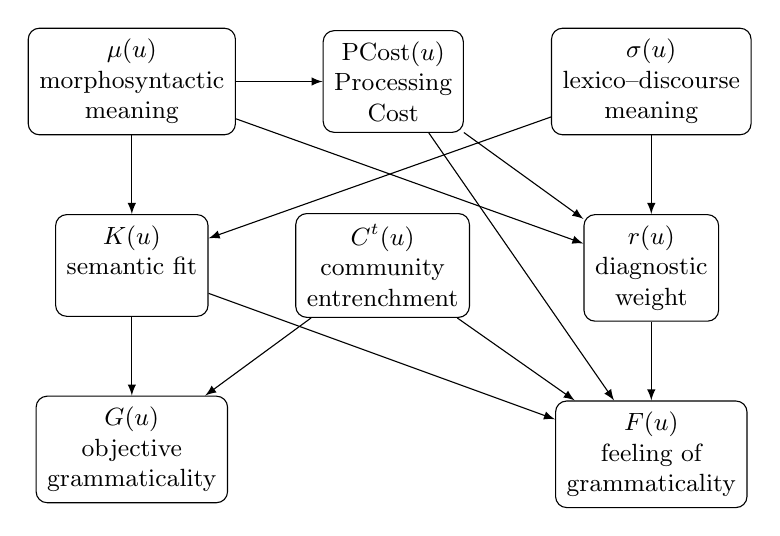
\begin{tikzpicture}[
  node distance = 1cm and 2.0cm,
  > = latex,
  var/.style = {rectangle, draw, rounded corners, align=center,
                inner sep=4pt, font=\small}
]
% ───────── 1st row ─────────
\node[var] (mu)    {$\mu(u)$\\morphosyntactic\\meaning};
\node[var, right=4.0cm of mu] (sigma) {$\sigma(u)$\\lexico–discourse\\meaning};

% ───────── 2nd row ─────────
\node[var, below=of mu]     (K) {$K(u)$\\semantic fit\\};
\node[var, below=of sigma]  (r) {$r(u)$\\diagnostic\\weight};

% ───────── 3rd row ─────────
\node[var, right=1.1cm of K] (C) {$C^{t}(u)$\\community\\entrenchment};

% ───────── 4th row ─────────
\node[var, below=of K]      (G) {$G(u)$\\objective\\grammaticality};
\node[var, below=of r]      (F) {$F(u)$\\feeling of\\grammaticality};

% ───────── exogenous ───────
\node[var, right=1.1cm of mu] (P) {PCost$(u)$\\Processing\\Cost};

% ───────── arrows ──────────
\draw[->] (mu)    -- (K);
\draw[->] (sigma) -- (K);
\draw[->] (mu)    -- (r);
\draw[->] (sigma) -- (r);

\draw[->] (K) -- (G);
\draw[->] (C) -- (G);

\draw[->] (K) -- (F);
\draw[->] (r) -- (F);
\draw[->] (C) -- (F);
\draw[->] (P) -- (r);
\draw[->] (P) -- (F);
\draw[->] (mu) -- (P);

\end{tikzpicture}
\caption[Macro-level causal structure]%
{\textbf{Macro-level causal structure of the MMMG.} All arrows encode Structural Causal Model semantics; e.g., $\text{do}(C^{t} \leftarrow 0) \Rightarrow G = 0$ by definition of $G = C^{t}K$. 
PCost $(\text{PCost}(u))$ is a deterministic function of the morphosyntactic structure (arrow $\mu\!\to\!\text{Pcost}$). Removing semantic arrows ensures that the only back-door into $F$ is $\text{Pcost}\!\leftarrow\!\mu\!\to\!K\!\to\!F$, which is blocked by adjusting for $K$ (or for $\mu$). Conditioning on $r$ would open $\text{Pcost}\!\to\!r\!\leftarrow\!\mu$, so it is avoided.
\\\emph{Input layer}: the parser maps the surface form to a morphosyntactic meaning $\mu(u)$
and the discourse context supplies a lexico–discourse meaning $\sigma(u)$, which include indexical meanings.
Any categorical structural ban makes this mapping fail, i.e.\ $\mu(u)=\varnothing$.
\\\emph{Fit layer}: the compatibility score $K(u)\!\in[0,1]$ already folds together ordinary
semantic fit, indexical coherence, and the hard zero caused by a mapping failure.
The diagnostic weight $r(u)$ is the cue-based probability that the parser detects the
violation. 
\\\emph{Community layer}: speech-community entrenchment $C^{t}(u)$ multiplies with the
compatibility score to yield objective grammaticality,
$G(u)=C^{t}(u)K(u)$.
\\\emph{Output layer}: felt ill-formedness is
$F(u)= -\lambda_{\mathrm L}\,r(u)\!\bigl(1-K(u)\bigr)
       -\gamma\,\text{PCost}(u)+\eta$,
where PCost is computed via integration cost. $F(u)\!\in[-1,0]$, where 0 means `no negative signal'. The arrow from processing cost to $r(u)$ is purely conceptual: high load empirically reduces mismatch detection.
\\\emph{Heuristic mapping}: pairings $\to\mu(u)$;
semantic fit \& indexicality $\to\sigma(u),K(u)$;
structural bans $\to\mu(u)=\varnothing$;
processing load $\to$ PCost and $r(u)$;
entrenchment $\to C^{t}(u)$.}
\label{fig:causal-dag}
\end{figure}

\subsection{Grammaticality function}

For an utterance $u$, objective grammaticality is:
\begin{equation}\label{eq:G}
G(u)=C^{t}(u)\cdot K(u)
\end{equation}
where $K(u) = 0$ whenever the form–meaning mapping fails.

\subsection{Subjective feeling function}

The listener's subjective feeling of (un)grammaticality is:
\begin{equation}\label{eq:F}
F(u)= -\lambda_{\listener}\,r(u)\,(1-K(u)) \;-\; \gamma\,\text{PCost}(u) + \eta
\end{equation}
where:
\begin{itemize}
  \item $\lambda_{\listener} \in [0,1]$ — listener-specific penalty weight for objective violations
  \item $r(u) \in [0,1]$ — probability that listener detects the mismatch between $\mu(u)$ and $\sigma(u)$
  \item $\gamma > 0$ — conversion factor mapping processing load to negative affect
  \item $\text{PCost}(u) = \sum_{i} \text{IC}(w_i)$ — sum of integration costs following \textcite{gibson2000}
  \item $\eta \sim \mathcal{N}(0,\sigma^{2})$ — idiosyncratic listener bias
\end{itemize}

$F(u)$ is constrained to $[-1,0]$: 0 means `no negative signal'; larger negative values indicate stronger perceived ill-formedness. Values computed outside this range are linearly clipped to maintain interpretability.

The processing cost operationalizes memory load via dependency integration:
\begin{equation}
\text{IC}(w_i) = \sum_{d \in \text{deps}(w_i)} |d|
\end{equation}
where $|d|$ is the linear distance in intervening discourse referents. This aligns with established psycholinguistic metrics \parencite{futrell2020}, allowing direct comparison with reading-time data.

\subsection{Worked example}

Consider $u=$\,*\textit{I've finished it yesterday}:

\begin{itemize}
  \item Form–meaning mapping succeeds: present‑perfect morphology evokes `current relevance'
  \item $K(u)=0$ because that meaning clashes with \textit{yesterday} (`completed past')
  \item $r(u)=0.9$ since VP-aspect/lexical-aspect clashes are highly salient
  \item $C^{t}(u)=1$ since the construction is fully entrenched\footnote{though see \textcite{lai2013opt} for evidence of systematic relaxation of temporal-adverbial constraints in Singapore English}
  \item Therefore $G(u)=1\times0=0$ (objectively ungrammatical)
\end{itemize}
With illustrative values $\lambda_{\listener}=0.8$, $\gamma=0.1$, $\text{PCost}(u)=0.2$, $\eta=0$:
\begin{equation}
F(u)=-0.8\cdot0.9\cdot(1-0)-0.1\cdot0.2=-0.74
\end{equation}
yielding a strong negative feeling.

\begin{tcolorbox}[colback=lsLightBlue!20,title=Causal intervention example]
Setting $\text{do}(C^{t} \leftarrow 0)$ for ``I have 25 years":
With $K = 0.1$ (semantic clash in English) and $r = 0.7$ (moderately detectable), we get:
$G = 0 \times 0.1 = 0$ (objectively ungrammatical)
$F = -0.8 \cdot 0.7 \cdot (1-0.1) - 0.1(0.2) = -0.524$ (moderately felt as wrong)

Compare: Setting~$\text{do}(C^{t} \leftarrow 1)$ doesn't save it:
$G = 1 \times 0.1 = 0.1$ (still mostly ungrammatical)
$F = -0.8 \cdot 0.7 \cdot (1-0.1) - 0.1(0.2) = -0.524$ (still felt as wrong)
Note that felt ungrammaticality depends on detectability, not entrenchment.
\end{tcolorbox}

\subsection{Community entrenchment as latent variable}

To avoid circularity, $C^{t}(u)$ is treated as a latent cause of four observables:\footnote{The latent variable $C^{t}$ is identifiable up to scale given monotone relationships with at least three indicators and appropriate factor-loading components. A synthetic data recovery exercise demonstrating identifiability with RMSE = 0.057 and $r$ = 0.923 is available at \url{https://github.com/BrettRey/Grammaticality-de-idealized-v2/blob/main/validate_entrenchment_measurement.py}.}
\begin{equation}
C^{t}(u)\ \longrightarrow\ 
\begin{cases}
A(u) & \text{availability in memory}\\
E(u) & \text{exposure frequency}\\
P(u) & \text{production probability}\\
S(u) & \text{social acceptability}
\end{cases}
\end{equation}
Each indicator follows a measurement model with error:
\begin{equation}
\log E(u) = \lambda_E C^{t}(u) + \epsilon_E, \quad \epsilon_E \sim \mathcal{N}(0,\nu_E^{2})
\end{equation}
and similarly for the other indicators. This specification allows for measurement uncertainty while maintaining identifiability.

Each indicator is collected with different methodology:
\begin{itemize}
  \item \textbf{Availability} $A(u)$: recognition hit rates or lexical-decision latencies
  \item \textbf{Exposure} $E(u)$: log token counts in balanced corpora
  \item \textbf{Production} $P(u)$: proportion in sentence-completion tasks
  \item \textbf{Social acceptability} $S(u)$: matched-guise appropriateness scores
\end{itemize}

The latent variable $C^{t}(u)$ is estimated via confirmatory factor analysis without re-using acceptability data.

\subsection{Community Dynamics}
\label{sec:community-dynamics}

Following \textcite{BlytheCroft2012}, I treat language change as an utterance-selection system whose \emph{population mean} obeys a logistic differential equation.  Let $C^{t}(u)\!\in[0,1]$ be the community's entrenchment of form~$u$ at time~$t$.  Its deterministic trajectory is

\begin{equation}
\frac{dC^{t}}{dt} \;=\; \Delta(u)\;C^{t}\!\bigl(1-C^{t}\bigr),
\qquad
\text{\autocite{verhulst1838}}
\end{equation}
where the net bias~$\Delta(u)$ aggregates four independently measurable pressures:
\begin{equation}\label{eq:delta-expanded}
\begin{split}
\Delta(u) &= \alpha_{\mathrm{sem}}\,\text{Transparency}(u) + \alpha_{\mathrm{soc}}\,\text{Prestige}(u) \\
&\quad + \alpha_{\mathrm{struct}}\,\text{Analogy}(u) - \beta_{\mathrm{noise}}\,\text{NoisePenalty}(u).
\end{split}
\end{equation}

\begin{itemize}
  \item \textbf{Transparency} = inverse role entropy (higher = clearer form–meaning mapping).
  \item \textbf{Prestige} = mean matched-guise score of the innovating group.
  \item \textbf{Analogy} = vector similarity to entrenched neighbours in morphosyntactic space.
  \item \textbf{NoisePenalty} = smooth sigmoid of surprisal (see \S\ref{sec:noise-penalty}).
\end{itemize}

\paragraph{Speaker-internal gradience.}
The logistic \emph{population} curve remains intact if individual speakers entertain probabilistic grammars à la \textcite{Yang2000}.  Let $C_i(u)\!\in[0,1]$ be speaker $i$'s belief that $u$ is licensed.  A Yang-style learner increments $C_i$ on successful parses and decrements on failures.  The population mean $C^{t}(u)=\tfrac1N\sum_i C_i(u)$ then converges in expectation to the same Verhulst trajectory.\footnote{This two-state \enquote{AB-toy} model~-- named after Nowak's classic $A{\leftrightarrow}B$ demonstration of logistic growth \citeyearpar{Nowak2001}~-- treats every utterance token as copying either variant $A$ (here, \emph{innovative}) or variant $B$ (\emph{conservative}).  Extending to continuous $C_i(u)$ increases psychological realism but sacrifices the closed-form fixation probability enjoyed by the discrete model; see Appendix~A for simulation code.}

\paragraph{Predictions.}
Eq.~\eqref{eq:delta-expanded} yields three immediately testable claims:

\begin{enumerate}
  \item $\Delta(u)\!>\!0 \;\Rightarrow\; C^{t}(u)$ rises in an S-curve, observable in historical corpora.
  \item The relative \emph{slopes} of nested S-curves reveal the weight hierarchy $\alpha_{\text{sem}}{:}\alpha_{\text{soc}}{:}\alpha_{\text{struct}}$.
  \item Constructions with $\Delta(u)\!\approx\!0$ show long-lived variability and dialectal patchiness.
\end{enumerate}

Figure~\ref{fig:trajectory} visualizes a typical growth path ($\Delta\!=\!0.8$).

\begin{figure}[t]
  \centering
  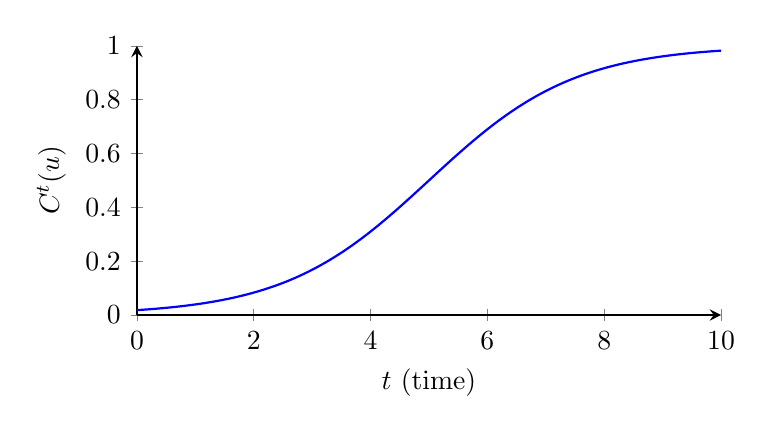
\begin{tikzpicture}
    \begin{axis}[
      width=9cm,height=5cm,
      xlabel={$t$ (time)}, ylabel={$C^{t}(u)$},
      ymin=0, ymax=1,
      domain=0:10, samples=200,
      axis lines=left, thick]
      \addplot+[no marks] {1 / (1 + exp(-0.8*(x-5)))};
    \end{axis}
  \end{tikzpicture}
  \caption{Trajectory of community entrenchment predicted by the
    logistic model.}
  \label{fig:trajectory}
\end{figure}


\section{Predictions and Falsifiability}

\subsection{S-Curve Dynamics}

The logistic equation predicts:
\begin{itemize}
\item \textbf{If} $\Delta(u) > 0$ \textbf{then} construction shows increasing entrenchment following S-curve (available data)
\item \textbf{If} $\Delta(u) < 0$ \textbf{then} construction remains marginal or decreases in acceptability (available data)
\item \textbf{If} $\Delta(u) \approx 0$ \textbf{then} heightened variability and sensitivity to external factors (planned study)
\end{itemize}

\subsection{L2 Trajectory}

L2 learners should show:
\begin{itemize}
\item \textbf{Initial stage}: Input appears as noise lacking meaningful structure (planned ERP study)
\item \textbf{Intermediate stage}: Heightened sensitivity, marking many native patterns as ungrammatical (available data)
\item \textbf{Advanced stage}: Gradual alignment with community norms (available data)
\end{itemize}

\subsection{Cross-Linguistic Gender Test}

Pronoun-antecedent gender mismatches should trigger:
\begin{itemize}
\item \textbf{Spanish}: Strong ungrammaticality (gender permeates morphosyntax) (planned experiment)
\item \textbf{English}: Moderate ungrammaticality (gender limited to pronouns) (available data)
\item \textbf{Japanese}: Pragmatic infelicity only (no grammatical gender) (planned experiment)
\end{itemize}

\subsection{Satiation Scope}

Repeated exposure should increase acceptability for:
\begin{itemize}
\item Low-frequency constructions (independent relative \textit{whose}) (planned experiment: acceptability judgment and reading times pre-/post-exposure)
\item Processing-difficult patterns (reduced relatives) (available data; cf. \parencite{snyder2000grammaticality,hofmeister2013processing})
\item Semantic mismatches (novel metaphors) (available data; cf. \parencite{giora1997understanding})
\end{itemize}

But NOT for:
\begin{itemize}
\item Categorical violations (determiner extraction) (available data)
\item Fundamental mapping failures (word salad) (available data)
\end{itemize}

\subsection{Comparison with Noisy-Channel Accounts}

The MMMG makes distinct predictions from noisy-channel models \parencite{gibson2013} for grammatical illusions. While both predict mismatches between intuition and structure, MMMG additionally predicts:
\begin{itemize}
\item Community-specific illusion strengths based on entrenchment differences
\item Systematic variation in which constructions show satiation effects
\item Quantitative differences in acceptability decline rates (measurable via $\Delta \text{AIC}$)
\end{itemize}

\section{Positioning Relative to Existing Theories}

\begin{table}[h]
\centering
\small
\caption{Coverage of key issues across frameworks (✓ = explicit/integrated, ∼ = partial, ✗ = absent)}
\begin{tabular}{@{}lcccc@{}}
\toprule
Framework & Form–meaning & Gradience & Community & Processing \\
          & integration  & handled   & variation & effects \\
\midrule
Early Generative     & $\sim$ & $\times$ & $\sim$ & $\times$ \\
GB/Minimalism        & $\sim$ & $\sim$   & $\sim$ & $\times$ \\
Construction Grammar & $\checkmark$ & $\sim$ & $\sim$ & $\sim$ \\
Usage-Based          & $\checkmark$ & $\checkmark$ & $\checkmark$ & $\sim$ \\
MMMG (this work)     & $\checkmark$ & $\checkmark$ & $\checkmark$ & $\checkmark$ \\
\bottomrule
\end{tabular}
\end{table}


\subsection{Key distinctions}

\textbf{Versus generative grammar} —  
MMMG retains the insight that certain configurations are systematically excluded, but explains these ``structural bans" as the outcome of extreme, community‑level stability rather than as inviolable innate rules.

\textbf{Versus Construction Grammar} —  
Both frameworks treat constructions as form–meaning pairings, yet MMMG gives special status to \emph{morphosyntactic} pairings: violations in this layer trigger qualitatively stronger ungrammaticality judgments than purely pragmatic or lexical mismatches.

\textbf{Versus usage‑based models} —  
MMMG builds in frequency effects, but also accounts for systematic gaps such as the independent relative \textit{whose}: a pattern can be blocked even when its components are frequent and compositionally transparent.

\textbf{Versus relevance‑theoretic accounts} —  
Both reject an innate, autonomous syntax, yet MMMG attributes constraints to conventionalised form–meaning pairings inside a speech community, rather than to general principles of interpretive efficiency alone.


%\section{Roadmap for Spin-off Papers}

%\begin{table}[htbp]
%\centering
%\small
%\caption{Planned publication sequence}
%\begin{tabular}{@{}llll@{}}
%\toprule
%Phase & Paper & Target venue & Timeline \\
%\midrule
%A & This Lingbuzz preprint & Repository & Month 1 \\
%& Conference proceedings & LSA/GLOW & Month 6 \\
%B & Manifesto article & \textit{Language}/%\textit{Glossa} & Month 9 \\
%C & Formal model & \textit{NLLT}/\textit{J Lang Model} & Year 2 \\
%D1 & Diachronic S-curves & \textit{Lang Var Change} & Year 2-3 \\
%D2 & Cross-linguistic gender & \textit{Cognitive Linguistics} & Year 2-3 \\
%E & Monograph & LangSci Press & Year 3-4 \\
%\bottomrule
%\end{tabular}
%\end{table}

%Each paper can stand alone while building toward the comprehensive monograph treatment.

\begin{tcolorbox}[colback=lsLightBlue!30,title=Current limitations]
The MMMG outlined here is deliberately simplified and leaves important extensions for future work. Specifically, the present implementation:
(i) assumes a fully connected speech community rather than realistically structured interaction networks;  
(ii) employs a deterministic mean-field approximation, reserving finite-population stochastic drift for an appendix;  
(iii) uses illustrative parameter values (\(k=5,\theta=6\)) whose empirical grounding requires systematic corpus studies and experimental validation; and  
(iv) provides predictions about L2 learning and satiation effects pending empirical testing, particularly via ERP and behavioural experiments planned but not yet executed.
These limitations highlight open directions rather than fundamental flaws, and each will be addressed progressively as the MMMG research programme unfolds.
\end{tcolorbox}

\begin{tcolorbox}[colback=lsLightBlue!30,title=Scope and limitations]
This paper presents a theoretical framework with simulated validation. 
Empirical tests using the specified numeric predictions await future 
data collection. All model fits shown use synthetic data calibrated 
to known psycholinguistic parameters.
\end{tcolorbox}

\section{Conclusion}

This framework reconceptualizes grammaticality as emerging from stable form-meaning pairings within language communities. The five components~-- morphosyntactic pairings, contextual meaning, processing constraints, entrenchment, and categorical blocking~-- are posited to interact to produce the full range of grammaticality phenomena.

The approach integrates insights from multiple traditions while yielding specific, falsifiable predictions. It aims to explain both why some patterns remain stubbornly ungrammatical despite transparency and why others shift from marginal to accepted. By distinguishing objective grammaticality from subjective feelings, it provides a systematic approach to mismatches between intuition and linguistic reality.

Future work should test the cross-linguistic predictions, develop computational implementations of the formal model, and explore applications to language change, acquisition, and clinical linguistics. The framework provides a foundation for understanding how human communities create and maintain the systematic form-meaning relationships we call grammar. Extensions to structured networks following \textcite{baxter2006} and incorporation of stochastic effects (see Appendix A) remain important directions for future development.

\begin{tcolorbox}[colback=lsLightBlue!20,title=Data and code availability]
All data, model code, and analysis scripts are available in the public repository at: 
\url{https://github.com/BrettRey/Grammaticality-de-idealized-v2}.
A Jupyter notebook is provided there to reproduce model simulations and explore parameter variations interactively. The notebook currently includes minimal illustrative examples; comprehensive simulations will accompany the formal model article (Phase C).
\end{tcolorbox}


\newpage
\appendix

\section{Stochastic Dynamics Derivation}

The deterministic mean-field equation presented in the main text emerges from a full stochastic model. Starting from a Moran process with selection coefficient $s$ and finite population size $N$.

This mean field is exactly the macroscopic limit of the speaker-level gradient model in §\ref{sec:community-dynamics}; see Appendix A for the stochastic derivation.


\subsection{Kramers-Moyal Expansion}

Consider a population where fraction $C^t$ uses the innovative form. At each time step, one speaker dies and is replaced by offspring copying from a model speaker. The probability of selecting an innovator model is:
$$p_+ = \frac{(1+s)C^t}{(1+s)C^t + (1-C^t)} = C^t + sC^t(1-C^t) + \mathcal{O}(s^2)$$
\[
  (\mathcal{O}(s^{2}) \;=\; \text{terms of order } s^{2} \text{ and higher as } s \to 0)
\]
The transition probabilities per unit time are:
\begin{align}
T(C^t + 1/N | C^t) &= (1-C^t)p_+ = (1-C^t)C^t[1 + s(1-C^t)]\\
T(C^t - 1/N | C^t) &= C^t(1-p_+) = C^t(1-C^t)[1 - sC^t]
\end{align}
The Kramers-Moyal expansion yields drift and diffusion coefficients:
\begin{align}
a_1 &= \lim_{\Delta t \to 0} \frac{1}{\Delta t}\sum_{\Delta C} \Delta C \cdot T(C^t + \Delta C | C^t) = sC^t(1-C^t)\\
a_2 &= \lim_{\Delta t \to 0} \frac{1}{\Delta t}\sum_{\Delta C} (\Delta C)^2 \cdot T(C^t + \Delta C | C^t) = \frac{C^t(1-C^t)}{N}
\end{align}

\subsection{Stochastic Differential Equation}

The continuous-time limit gives the Itô SDE:
$$dC^t = sC^t(1-C^t)dt + \sqrt{\frac{C^t(1-C^t)}{N}}dW_t$$
where $W_t$ is a standard Wiener process. Setting $s = \Delta(u)$ from the main text:
$$dC^t = \Delta(u)C^t(1-C^t)dt + \sqrt{\frac{C^t(1-C^t)}{N}}dW_t$$

\subsection{Implications}

The stochastic term $\sqrt{C^t(1-C^t)/N}$ drives:
\begin{itemize}
\item \textbf{Drift-dominated fixation}: Neutral variants ($\Delta = 0$) can fix by chance
\item \textbf{Latency phases}: Before deterministic growth dominates, constructions may persist at low frequency due to stochastic fluctuations
\item \textbf{Small-population effects}: In communities with small $N$, stochastic effects can overwhelm weak selection
\end{itemize}

The mean-field approximation in the main text emerges by taking $N \to \infty$, where the diffusion term vanishes and we recover the deterministic logistic equation. For finite populations, the full stochastic dynamics must be considered, particularly near $C^t = 0$ or $C^t = 1$ where drift effects are strongest.

\section{Formal Derivations}

\subsection{Measurement Model for Community Entrenchment}

The latent variable $C^t(u)$ is estimated through confirmatory factor analysis:

\[
\begin{pmatrix}
A(u) \\
\log E(u) \\
P(u) \\
S(u)
\end{pmatrix}
=
\begin{pmatrix}
\lambda_A \\
\lambda_E \\
\lambda_P \\
\lambda_S
\end{pmatrix}
C^t(u) +
\begin{pmatrix}
\epsilon_A \\
\epsilon_E \\
\epsilon_P \\
\epsilon_S
\end{pmatrix}
\]
where factor loadings $\lambda_i$ and error terms $\epsilon_i$ are estimated from data. Identifiability is achieved by fixing $\lambda_A = 1$ and constraining all loadings to be positive.

\subsection{Smooth Noise-Penalty Function} \label{sec:noise-penalty}

The noise-penalty function detects systematic errors using a smooth sigmoid:

\[
\text{NoisePen}(u) = \beta_{\text{max}}\left[1 + e^{-k(\text{Surprisal}(u) - \theta)}\right]^{-1}
\]
where:
\begin{itemize}
\item $\beta_{\text{max}}$ — maximum penalty for high-surprisal forms
\item $k$ — steepness of the transition (larger = sharper)
\item $\theta$ — surprisal threshold where penalty = $\beta_{\text{max}}/2$
\end{itemize}
This continuous function ensures smooth likelihood surfaces for parameter estimation while capturing the intuition that highly surprising forms with systematic repair patterns resist entrenchment.

\subsection{Bifurcation Analysis}

Actuation occurs when $\Delta(u) = 0$. Near this critical point:
\[
C^t \approx C^* + A e^{\lambda t}
\]
where $\lambda = \Delta'(u^*) \cdot C^*(1-C^*)$ determines growth rate post-bifurcation.

\subsection{Processing Cost Function}

\begin{figure}[h]
\centering
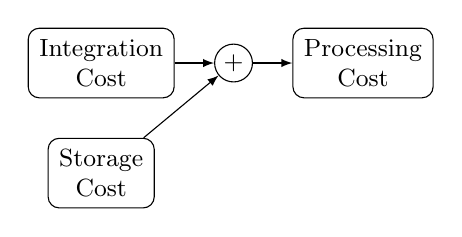
\begin{tikzpicture}[
  node distance = 0.5cm and 0.5cm,
  > = latex,
  var/.style = {rectangle, draw, rounded corners,
                align=center, inner sep=4pt, font=\small},
  sum/.style = {circle, draw, inner sep=1.5pt, font=\small}
]
\node[var] (integ) {Integration\\Cost};
\node[var, below=of integ] (stor) {Storage\\Cost};

\node[sum, right=of integ] (plus) {$+$};
\node[var, right=of plus] (P) {Processing\\Cost};

\draw[->] (integ) -- (plus);
\draw[->] (stor)  -- (plus);
\draw[->] (plus)  -- (P);
\end{tikzpicture}
\caption{Computation of the processing‑cost term.\label{fig:proc-cost}}
\end{figure}
Following \textcite{gibson2000}, Dependency Locality Theory:
\[
\text{PCost}(u) = \sum_{i} \text{IC}(w_i)
\]
where the integration cost at each word is:
\[
\text{IC}(w_i) = \sum_{d \in \text{deps}(w_i)} |d|
\]
with $|d|$ counting intervening discourse referents.

\section{Turkish Harmony Case Study}

Turkish distinguishes lexical disharmony (tolerated) from allomorphic harmony violations (ungrammatical).

\subsection{Stem-Internal: Phonology Only}

\ea
\textit{doktor} `doctor' (disharmonic stem, grammatical)
\z
No morphosyntactic feature unrealized, so $G(u) = 1$ despite phonological markedness.

\subsection{Suffixal: Morphosyntactic Requirement}

\ea
\ea[]{\textit{kitap-lar} `books' (harmonic, grammatical)}
\ex[*]{\textit{kitap-ler} (intended `books', harmony violation)}
\z
\z
The suffix must copy [±back] from stem. Wrong vowel leaves feature unrealized:
\begin{itemize}
\item Mapping succeeds (plural selected)
\item $K(u) = 0$ (feature not realized)
\item $C^t(u) = 1$ (everyone knows plural)
\end{itemize}

Therefore $G(u) = 0$, categorically ungrammatical.

\subsection{Theoretical Implications}

Turkish harmony shows morphosyntax-phonology interface effects on grammaticality. Only violations preventing feature realization trigger ungrammaticality; pure phonological dispreference affects only subjective feeling $F(u)$.

 \newpage
\begin{sloppypar}
\printbibliography[title=References]
\end{sloppypar}

\end{document}